%%%%%%%%%%%%%%%%%%%%%%%%%%%%%%%%%%%%%%%%%
% Beamer Presentation
% LaTeX Template
% Version 1.0 (10/11/12)
%
% This template has been downloaded from:
% http://www.LaTeXTemplates.com
%
% License:
% CC BY-NC-SA 3.0 (http://creativecommons.org/licenses/by-nc-sa/3.0/)
%
%%%%%%%%%%%%%%%%%%%%%%%%%%%%%%%%%%%%%%%%%

%----------------------------------------------------------------------------------------
%	PACKAGES AND THEMES
%----------------------------------------------------------------------------------------

\documentclass{beamer}

\mode<presentation> {

% The Beamer class comes with a number of default slide themes
% which change the colors and layouts of slides. Below this is a list
% of all the themes, uncomment each in turn to see what they look like.

% \usetheme{default}
%\usetheme{AnnArbor}
%\usetheme{Antibes}
%\usetheme{Bergen}
% \usetheme{Berkeley}
% \usetheme{Berlin}
%\usetheme{Boadilla}
%\usetheme{CambridgeUS}
%\usetheme{Copenhagen}
%\usetheme{Darmstadt}
%\usetheme{Dresden}
%\usetheme{Frankfurt}
%\usetheme{Goettingen}
%\usetheme{Hannover}
%\usetheme{Ilmenau}
%\usetheme{JuanLesPins}
%\usetheme{Luebeck}
\usetheme{Madrid}
%\usetheme{Malmoe}
%\usetheme{Marburg}
%\usetheme{Montpellier}
% \usetheme{PaloAlto}
%\usetheme{Pittsburgh}
%\usetheme{Rochester}
% \usetheme{Singapore}
%\usetheme{Szeged}
% \usetheme{Warsaw}

% As well as themes, the Beamer class has a number of color themes
% for any slide theme. Uncomment each of these in turn to see how it
% changes the colors of your current slide theme.

%\usecolortheme{albatross}
%\usecolortheme{beaver}
%\usecolortheme{beetle}
%\usecolortheme{crane}
%\usecolortheme{dolphin}
%\usecolortheme{dove}
%\usecolortheme{fly}
%\usecolortheme{lily}
%\usecolortheme{orchid}
%\usecolortheme{rose}
%\usecolortheme{seagull}
%\usecolortheme{seahorse}
%\usecolortheme{whale}
%\usecolortheme{wolverine}

%\setbeamertemplate{footline} % To remove the footer line in all slides uncomment this line
%\setbeamertemplate{footline}[page number] % To replace the footer line in all slides with a simple slide count uncomment this line

%\setbeamertemplate{navigation symbols}{} % To remove the navigation symbols from the bottom of all slides uncomment this line
}

\usepackage{graphicx} % Allows including images
\graphicspath{img}
\usepackage{booktabs} % Allows the use of \toprule, \midrule and \bottomrule in tables
\usepackage[colorlinks]{hyperref}

%----------------------------------------------------------------------------------------
%	TITLE PAGE
%----------------------------------------------------------------------------------------

\title[Intro to RL]{Basics of reinforcement learning} % The short title appears at the bottom of every slide, the full title is only on the title page

\author{Yixin Lin} % Your name
\institute[Duke] % Your institution as it will appear on the bottom of every slide, may be shorthand to save space
{
Duke University \\ % Your institution for the title page
\medskip
\textit{yixin.lin@duke.edu} % Your email address
}
\date{February 15, 2017} % Date, can be changed to a custom date

\begin{document}

\begin{frame}
\titlepage % Print the title page as the first slide
\end{frame}

\begin{frame}
\frametitle{Overview} % Table of contents slide, comment this block out to remove it
\tableofcontents % Throughout your presentation, if you choose to use \section{} and \subsection{} commands, these will automatically be printed on this slide as an overview of your presentation
\end{frame}

\section{Introduction}

\begin{frame}
\frametitle{Introduction}
\begin{itemize}
  \item Picking the right problem is \textit{hard}
  \item Capturing the right abstraction level: all the relevant details, none of the irrelevant ones
  \item Three (extremely general!) types of tasks in machine learning
    \begin{itemize}
      \item Supervised learning
      \item Unsupervised learning
      \item Reinforcement learning
    \end{itemize}

\end{itemize}
\end{frame}

\begin{frame}
\frametitle{Introduction}
\begin{itemize}
  \item Reinforcement learning is the problem of \textit{sequential decision making in dynamic environment}
  \item Goal: capture the most important aspects of an agent making decisions
    \begin{itemize}
      \item Input (sensing the state of the environment)
      \item Action (choosing to affect on the environment)
      \item Goal (prefers some states of the environment over others)
    \end{itemize}
  \item This is \textit{incredibly} general
  \item Examples
    \begin{itemize}
      \item Robots (and their components)
      \item Games
      \item Better A/B testing
      \item Most importantly, \textbf{you}!
    \end{itemize}
\end{itemize}
\end{frame}

\section{Difficulties}

\begin{frame}
\frametitle{Difficulties}
\begin{itemize}
  \item Curse of dimensionality: too many choices!
  \item Stochasticity, and more generally, uncertainty: what do I do?
  \item Reward choice: what do I care about?
  \item \textit{Credit assignment}: what did I do wrong?
\end{itemize}
\end{frame}

\section{Elements of reinforcement learning}

\begin{frame}
  \frametitle{Elements of reinforcement learning}
  \begin{itemize}
    \item Policy: how I act in a given situation
    \item Reward signal: pain and pleasure at the moment
    \item Value function: total amount of happiness from now until I die
  \end{itemize}
\end{frame}


\section{The Markov Decision Process (MDP)}

\begin{frame}
  \frametitle{The Markov Decision Process (MDP)}
  \begin{itemize}
    \item $S$: set of possible \textbf{states} of the environment
    \begin{itemize}
      \item $p(s_0), s_0 \in S$: a distribution over initial state
      \item Markov property: we assume that the current state summarizes everything we need to remember
    \end{itemize}
    \item $A$: set of possible \textbf{actions}
    \begin{itemize}
      \item $P_{sa}(\cdot)$: state transitions, for each state $s$ and action $a$
    \end{itemize}
    \item $R: S \rightarrow \mathbb{R}$: \textbf{reward}
    \begin{itemize}
      \item $\gamma \in [0,1]$: discount factor
    \end{itemize}
  \end{itemize}
\end{frame}

\begin{frame}
  \frametitle{The Markov Decision Process (MDP)}
  \begin{itemize}
    \item $\pi$: a policy (what action to do, given a state)
    \item $V^\pi(s) = E_\pi[\sum_{i=0}^\infty \gamma^i R(s_i)]$
    \begin{itemize}
      \item How good is a state, given a policy?
    \end{itemize}
  \item $Q^\pi(s, a)$
    \begin{itemize}
      \item How good is an action at a state, given a policy?
    \end{itemize}
  \item More realistic: Partially Observed MDPs (POMDPs), where state is not directly observed but affects observations
  \end{itemize}

\end{frame}

\section{Techniques for solving RL problems}

\begin{frame}
  \frametitle{Techniques for solving RL problems}
  \begin{itemize}
      \item Dynamic programming
      \item Temporal difference (TD) learning
      \item Q-learning: find the Q function (how good is the action?)
      \item Policy gradients: optimize the policy directly
      \item Deep RL: use deep neural networks as function approximators

        \begin{itemize}
          \item Deep Q-learning
          \item Policy gradients: learn a policy directly
        \end{itemize}
  \end{itemize}
\end{frame}

\section{Recent successes}

\begin{frame}
  \frametitle{Recent successes: Atari}

  \begin{figure}
    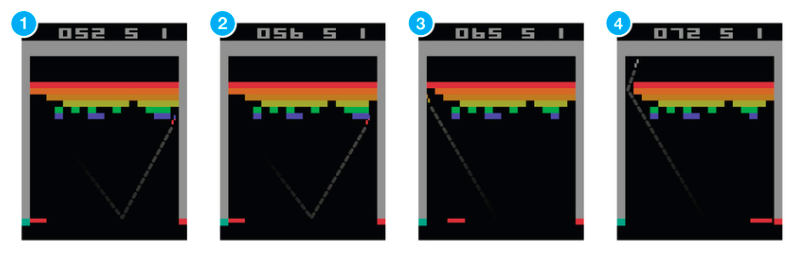
\includegraphics[width=0.6\linewidth]{img/atari.png}
  \end{figure}
  \begin{itemize}
    \item \href{http://www.nature.com/nature/journal/v518/n7540/full/nature14236.html}{``Human-level control through deep reinforcement learning'', Mnih et al.}
  \end{itemize}
\end{frame}

\begin{frame}
  \frametitle{Recent successes: AlphaGo}

  \begin{figure}
    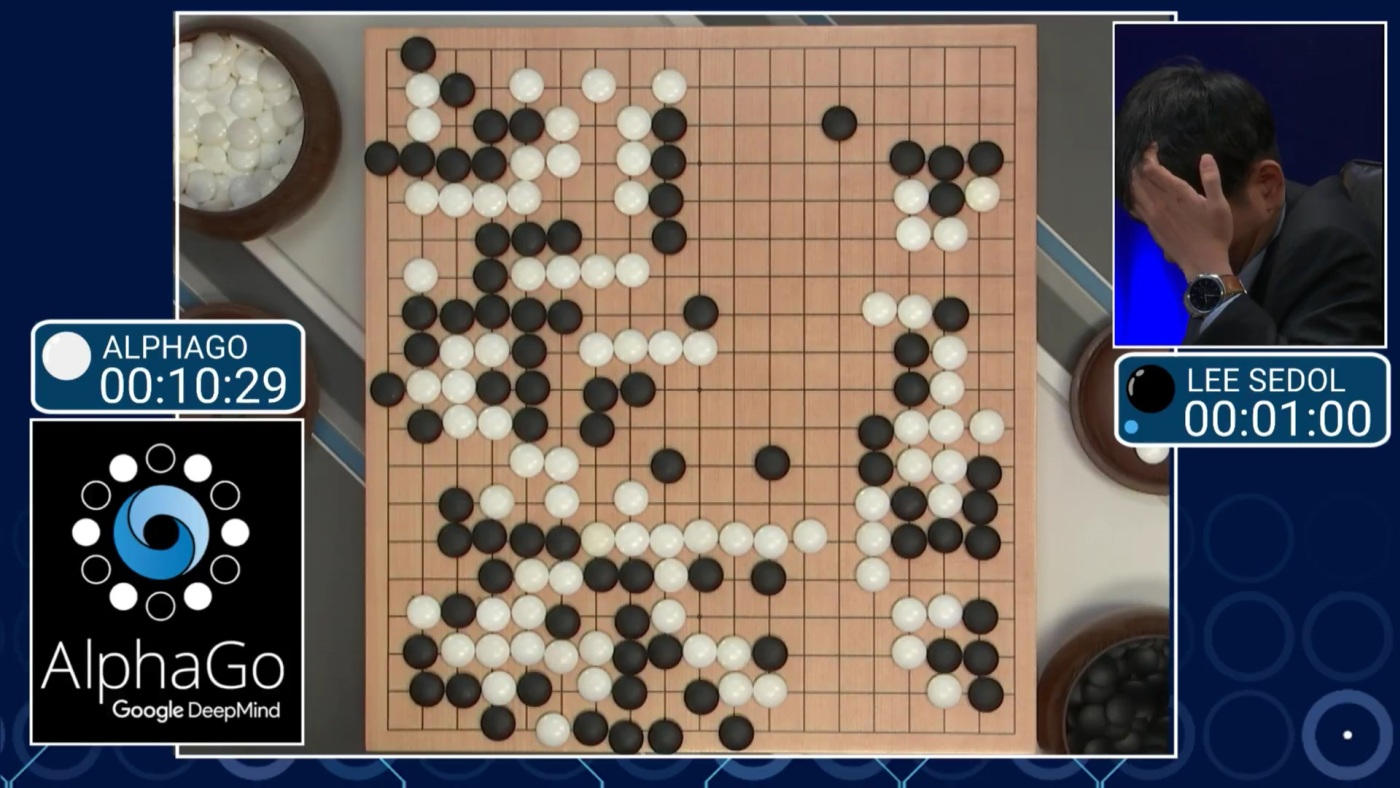
\includegraphics[width=0.6\linewidth]{img/alphago.jpg}
  \end{figure}
  \begin{itemize}
    \item \href{http://www.nature.com/nature/journal/v518/n7540/full/nature14236.html}{``Mastering the game of Go with deep neural networks and tree search'', Silver et al.}
  \end{itemize}
\end{frame}

\section{Failure modes}

\begin{frame}
  \frametitle{Failure modes}

  \begin{figure}
    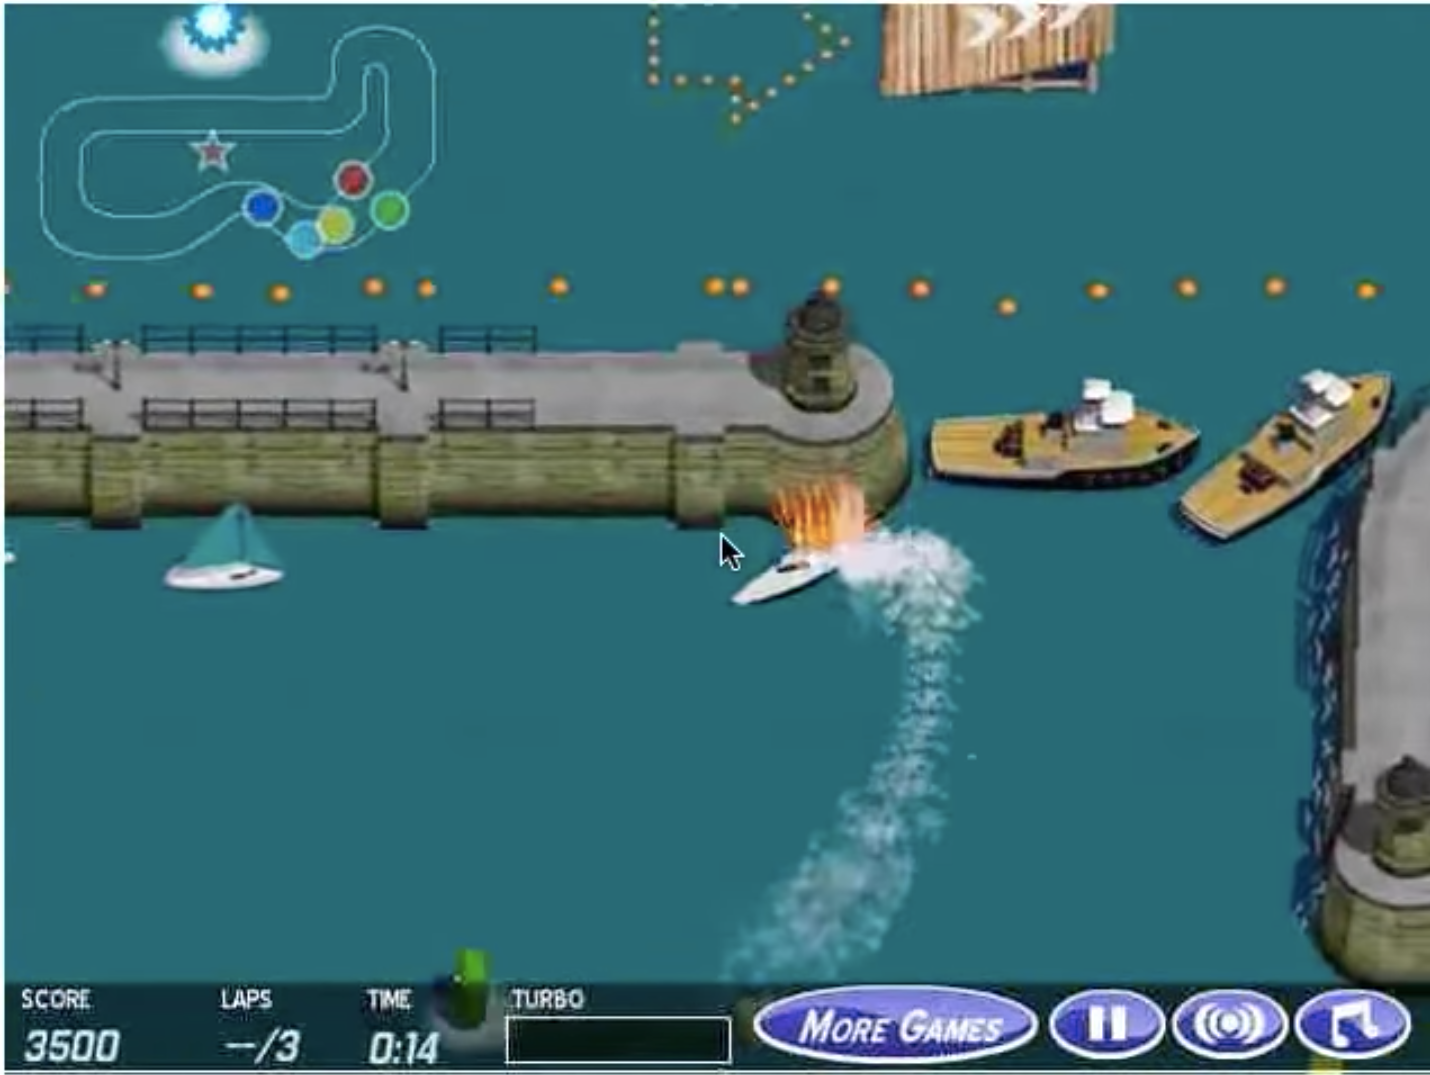
\includegraphics[width=0.4\linewidth]{img/coastrunners.png}
  \end{figure}
  \begin{itemize}
    \item \href{https://www.youtube.com/watch?v=tlOIHko8ySg}{Misspecifying reward functions} (\href{https://openai.com/blog/faulty-reward-functions/}{OpenAI blog})
    \item \href{https://openai.com/blog/concrete-ai-safety-problems/}{Concrete AI safety problems}
      \begin{itemize}
        \item Safe exploration (don't destroy the environment or itself)
        \item Changing environments and data (fail gracefully when data changes)
        \item Avoid negative side-effects (can't explicitly describe every bad behavior)
        \item Avoid wireheading (reward signals are faulty)
        \item Scalable oversight (when feedback and oversight is expensive)
      \end{itemize}
  \end{itemize}
\end{frame}

\section{AI safety problems}

\begin{frame}
  \frametitle{AI safety problems}

  \begin{itemize}
    \item Recent papers
    \begin{itemize}
      \item \href{https://arxiv.org/abs/1606.06565}{``Concrete problems in AI safety'', Amodei et al.}
      \item \href{https://intelligence.org/files/Interruptibility.pdf}{``Safely interruptible agents'', Orseau and Armstrong}
    \end{itemize}
  \item Organizations
    \begin{itemize}
      \item Machine intelligence research institute (MIRI)
      \item Future of humanity institute (FHI)
      \item Partnership on AI
        \begin{itemize}
          \item AAAI, ACLU, Amazon, Google (DeepMind), Facebook, IBM, Microsoft, Apple, OpenAI)
        \end{itemize}
    \end{itemize}
  \end{itemize}
\end{frame}


\begin{frame}
\Huge{\centerline{Thanks!}}

\Large{\centerline{Resources and references: \href{yixinlin.net/intro-rl}{yixinlin.net/intro-rl}}}

\end{frame}

%----------------------------------------------------------------------------------------

\end{document} 
